\section{Database and selection of test subjects}
DB given samples given


\section{Morphing of Faces}
Creating morphes can
\subsection{Automatic morphing}

\subsubsection{Results}

\subsection*{Manual morphing}
In contrast to the automatic face morphing approach, manual morphing is discussed in this section. 

To achieve morphes, the open source software GNU Image Manipulation Software (GIMP) (Version 2.8.16)with the GIMP Animation Package (GAP) (Version 2.6) was selected for this paper. Morphing with GAP follows the simple approach of manually placing connected landmarks at characterizing points in both faces. The algorithm shifts the landmarks from face one to face two. In addition to this the color of the skin is transmitted. 

\subsubsection*{Morphing setup}
For the test samples 100 - 125 landmarks were placed, depending on the face characteristics. The output contains a sequence of 30 photos which show different stages of the morphing procedure. A manual post production of the morphed was not necessary. 

\subsubsection*{Results}

\begin{figure} 
	\centering
	\subfloat[Subject 1]{%
		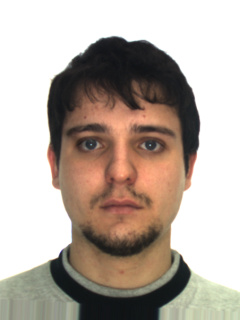
\includegraphics[width=0.45\linewidth]{Resources/p1.jpg}}
	\label{1a}\hfill
	\subfloat[Morph no. 5]{%
		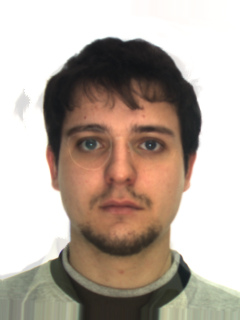
\includegraphics[width=0.45\linewidth]{Resources/m1.jpg}}
	\label{1b}\\
	\subfloat[Morph no. 15]{%
		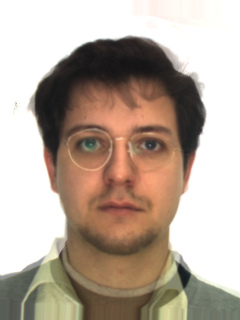
\includegraphics[width=0.45\linewidth]{Resources/m2.jpg}}
	\label{1c}\hfill
	\subfloat[Morph no. 25]{%
		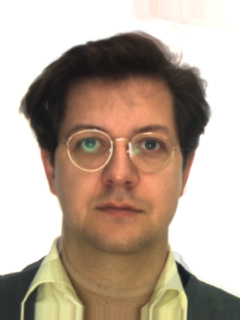
\includegraphics[width=0.45\linewidth]{Resources/m3.jpg}}
	\label{1d}\hfill
	\subfloat[Subject 2]{%
		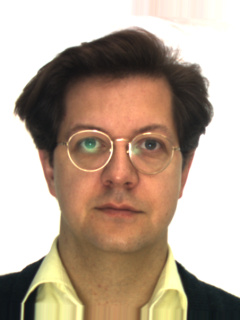
\includegraphics[width=0.45\linewidth]{Resources/p2.jpg}}
	\label{1e} 
	\caption{Example of two ICAO compliant photos (1a and 1e) and morphs at stage 5 (1b), 15 (1c) and 25 (1d)}
	\label{fig1} 
\end{figure}
.
\todo[inline]{Detailed description of the morphs}